\graphicspath{{content/chapters/4_Methodology/figures/}}
\chapter{Methodology}\label{chp:methodology}

This chapter details the technical implementation of the proof-of-concept system. The
methodology is structured around the four primary project objectives, transitioning from
physical marker design to the final kinematic extraction engine. Critically, each phase was
designed not in isolation but in direct response to the failure modes introduced by the
preceding phase: the marker design constrains what the detector must handle, the detector's
output feeds the scale calibration, and the calibration underpins the accuracy of every
kinematic metric. The decisions documented here are therefore presented as a chain of
engineering arguments rather than a sequence of independent implementation choices. The code for the entire pipeline is available in the project's GitHub repository, with links provided in Appendix~\ref{chp:code_repository}.

% ============================================================
\section{Marker Design and Visibility}\label{sec:marker-design}
% ============================================================

Objective~\ref{obj:marker_design} required a modular marker design capable of withstanding the
high-turbulence environment of a swimming pool while remaining identifiable under varying
refractive conditions.

The lack of existing documentation on underwater marker design for \gls{cv} applications
necessitated an iterative prototyping approach. This led to the decision to create a modular
design for a 3D-printed marker that could be easily set up along the lane. The final design, as
shown in Figure~\ref{fig:marker-design}, consists of high-contrast, alternating black and white
segments, which seamlessly screw into one another. This decision to use a modular design allowed
us to test various configurations, mainly how many segments to stack, effectively altering the
height of the marker.

\begin{figure}[htbp]
    \centering
    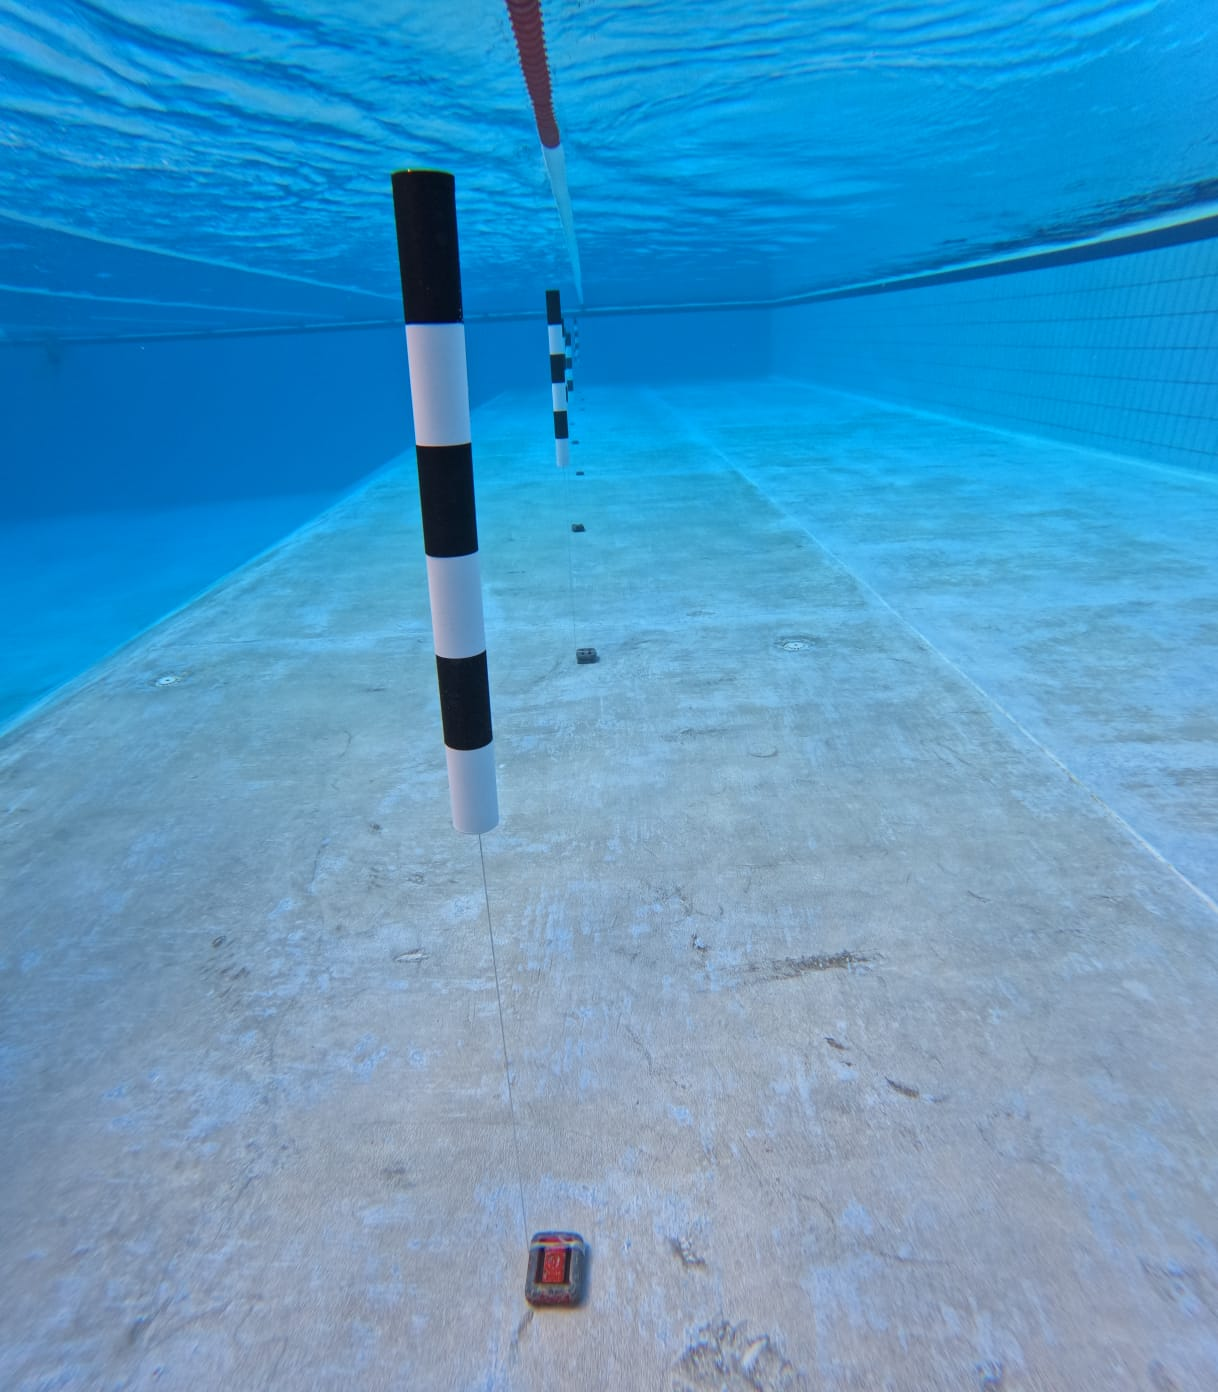
\includegraphics[width=0.6\textwidth,keepaspectratio]{marker_design.jpg}
    \caption{An image of the final marker design in use.\label{fig:marker-design}}
\end{figure}

\subsection{Pattern Selection: High-Contrast Binary Alternation}

The choice of an alternating black-and-white pattern over coloured or single-colour designs was
motivated by the specific optical failure modes of the aquatic environment. Coloured markers
suffer from wavelength-dependent attenuation: water selectively absorbs red and orange
wavelengths within the first few metres of depth, causing a progressive blue-shift that
desaturates warm tones and renders chromatic patterns highly variable across different pool
depths and lighting conditions. Fluorescent pool lighting compounds this problem by introducing
a spectrally narrow illuminant that can cause metameric failure, where colours that appear
distinct under natural light become perceptually indistinguishable under artificial spectra.
Monochromatic high-contrast patterns sidestep these failure modes entirely because detection
relies on luminance gradients rather than hue. A binary pattern of maximum contrast, such as pure
black against pure white, retains a large gradient even after the global contrast reduction
caused by water's scattering coefficient and the distorting effects of refraction at the
air-water interface~\cite{agrawal2012theory}.

The alternating structure, rather than a solid single-colour cylinder, was chosen for two
further reasons. First, a solid black cylinder placed near a dark pool floor or against a dark
swimsuit provides insufficient contrast for reliable edge detection, whereas an alternating
pattern creates multiple distinct transitions detectable by gradient-based feature extraction
regardless of the local background. Second, the periodic alternation constitutes a unique
visual signature that distinguishes the marker from other cylindrical objects present in the
scene, most notably lane rope buoys, which are typically uniform in colour along their length.
This distinction is exploited implicitly by the downstream detector, which learns that the
alternating pattern is a necessary characteristic of a valid detection.

\subsection{Physical Form Factor: Cylindrical and 3D-Printed}

Off-the-shelf calibration targets such as chequerboard boards or ArUco markers were considered
as alternatives. These planar targets are well-characterized in the literature~\cite{hartley2003multiple}
and are the standard choice for metric calibration in controlled laboratory settings. However,
they present a fundamental geometric limitation in the poolside context: their detectability
is highly sensitive to viewing angle. At the oblique angles typical of handheld poolside
footage, a flat board subtends a narrow projected area and its corner features become
unreliable, degrading calibration accuracy precisely in the conditions under which the system
must operate. No commercially available waterproof, poolside-mountable calibration target of
appropriate scale was identified during the design phase, reinforcing the case for a bespoke
solution.

A cylindrical form was selected because rotational symmetry about the vertical axis guarantees
that the marker presents a geometrically consistent cross-section from any horizontal viewing
direction. Whether the operator films from directly to the side or at a moderate angle, the
apparent width of the cylinder changes only by the cosine of the viewing angle, and within the
moderate angular range achievable from a poolside position, this variation is small. The
decision to 3D-print the markers allowed rapid iteration over design parameters and ensured
the final geometry was precisely controlled.

Each segment is 10 cm in height, with a 5 cm diameter, and the alternating pattern provides a
unique visual signature that can be reliably detected by \gls{cv} algorithms. The design
also incorporates a screw mechanism that allows for easy assembly and disassembly, enabling
quick setup along the lane for calibration purposes. This modularity not only facilitates
testing different configurations but also ensures that the markers can be easily transported
and stored when not in use. The 10 cm segment height was determined by the requirement that
the marker subtend a sufficient number of pixels to be reliably detected at the maximum
anticipated operating distance: at a camera-to-marker distance of approximately two to three
metres, a 10 cm feature projects to roughly 50 pixels at a 1080p resolution, which is
sufficient for a \gls{yolo}-family one-stage detector to localize accurately. A smaller segment
height would have reduced this pixel count below the threshold of reliable detection, while a
larger height would have increased physical mass and the risk of the marker toppling in
turbulent conditions.

\subsection{Marker Spacing and Empirical Calibration}

The spacing between the markers was determined based on multiple tests, which revealed that an
interval of 2.5 m provided a good balance between visibility and the number of markers required
for accurate calibration. This spacing allows for sufficient coverage along the lane while
minimizing the number of markers needed, which is crucial for minimizing setup time and
complexity.

The spacing decision involved explicit consideration of the failure modes at both extremes. A
1 m spacing would increase the total number of markers required to cover a 25 m or 50 m lane,
substantially raising setup complexity and the likelihood of inter-marker occlusion as the
swimmer's body passes between the camera and multiple adjacent markers simultaneously. A 5 m
spacing would reduce the probability of two or more markers being simultaneously visible within
the camera's field of view at any given moment, which is the minimum condition for a stable
pixel-to-metre ratio estimate. With only a single marker visible, no inter-marker distance can
be computed, and the scale calibration must fall back to a carried-forward estimate from the
previous valid frame, introducing temporal staleness. The 2.5 m spacing was identified through
empirical trials as the minimum spacing at which at least two markers reliably remained within
the camera's field of view throughout the swimmer's traversal of the monitored segment, given
the focal length and field of view of the camera used in the trials. This provides a stable
baseline for pixel-to-metre ratio estimation at every frame, minimizing reliance on the
carry-forward fallback described in Section~\ref{sec:scale-extraction}.

\subsection{Prototyping Iterations}

Early prototypes explored solid single-colour cylinders, different diameters, and varying
numbers of stacked segments. Solid-colour prototypes exhibited the contrast failure modes
described above under pool conditions, particularly when the camera position placed the marker
against a similarly toned background. Markers with a diameter smaller than 5 cm proved
difficult to detect reliably beyond 2 m, while larger diameters increased buoyancy and
required heavier weighting to remain upright. These observations collectively converged on the final configuration: a 5 cm diameter cylinder with 10 cm alternating segments, spaced at 2.5 m intervals.

% ============================================================
\section{Dataset Generation and \gls{mitl} Annotation}\label{sec:dataset-generation}
% ============================================================

To address Objective~\ref{obj:dataset_creation}, necessitated by the lack of annotated underwater datasets, a
\gls{mitl} workflow was developed. This phase utilized foundation models to
automate the labelling process for the downstream \gls{yolo26} detector. The entire dataset creation
pipeline is visualized in Figure~\ref{fig:training_pipeline}.

\begin{figure}[htbp]
    \centering
    % Resizes the diagram to fit the width of the page text perfectly
    \resizebox{\textwidth}{!}{
        \begin{tikzpicture}[
                % Define styles for the boxes and lines
                base/.style = {rectangle, rounded corners, draw=black, thick, minimum width=3.5cm, minimum height=1.2cm, text centered, font=\sffamily\small, text width=3.2cm, fill=white},
                decision/.style = {diamond, aspect=1.5, draw=black, thick, text centered, font=\sffamily\footnotesize, text width=2.2cm, fill=white, inner sep=0pt},
                terminal/.style = {rectangle, rounded corners=0.6cm, draw=black, thick, minimum width=3.5cm, minimum height=1.2cm, text centered, font=\sffamily\small, text width=3.2cm, fill=green!5},
                arrow/.style = {thick, ->, >=stealth},
                phase_arrow/.style = {thick, ->, >=stealth, blue!80!black, rounded corners},
                phase_box/.style = {draw=gray!80, thick, dashed, inner sep=12pt, fill=gray!5, rounded corners}
            ]

            % ---------------------------------------------------
            % PHASE 0 NODES (Column 1)
            % ---------------------------------------------------
            \node (A) [base] {Extract Video Frames};
            \node (B) [base, below=0.5cm of A] {Initialize CUDA \& SAM2 Model};
            \node (C) [base, below=0.5cm of B] {Draw Bounding Boxes using an intactive GUI};
            \node (D) [base, below=0.5cm of C] {Save Initial Marker Coordinates \& Classes};

            % ---------------------------------------------------
            % PHASE 1 NODES (Column 2)
            % ---------------------------------------------------
            % Increased spacing to 1.6cm to make room for arrows between columns
            \node (E) [base, right=1.6cm of A] {Run SAM2 Tracking over Video Chunk};
            \node (F) [base, below=0.5cm of E] {Generate Object Masks for Each Frame};
            \node (G) [base, below=0.5cm of F] {Convert Masks to Bounding Boxes};
            \node (H) [base, below=0.5cm of G] {Export Images \& Labels into YOLO Format};

            % ---------------------------------------------------
            % PHASE 1.5 NODES (Column 3)
            % ---------------------------------------------------
            \node (I) [base, right=1.6cm of E] {Analyze Box Dimensions};
            \node (J) [base, below=0.5cm of I] {Filter Outlier Boxes via IQR Method};
            \node (K) [base, below=0.5cm of J] {Train Lightweight YOLOv8n (A/B Testing)};
            \node (L) [base, below=0.5cm of K] {Compare Loss, mAP \& Visual Results};
            \node (M) [decision, below=0.4cm of L] {Select Best Dataset};

            % ---------------------------------------------------
            % PHASE 2 NODES (Column 4)
            % ---------------------------------------------------
            \node (N) [base, right=1.6cm of I] {Spot-Check Final Labels Visually};
            \node (O) [base, below=0.5cm of N] {Inject Hard Negatives (Background frames)};
            \node (P) [base, below=0.5cm of O] {Write YOLO Configuration YAML};
            \node (Q) [base, below=0.5cm of P] {Execute Training with Best Dataset};
            \node (R) [terminal, below=0.5cm of Q] {Save the best weights to \texttt{best.pt}};

            % ---------------------------------------------------
            % DRAW PHASE BACKGROUND BOXES
            % ---------------------------------------------------
            \begin{scope}[on background layer]
                \node (P0) [phase_box, fit=(A) (D), label={[font=\sffamily\bfseries]above:Setup \& Annotation}] {};
                \node (P1) [phase_box, fit=(E) (H), label={[font=\sffamily\bfseries]above:Tracking \& Export}] {};
                \node (P15) [phase_box, fit=(I) (M), label={[font=\sffamily\bfseries]above:Dataset Optimization}] {};
                \node (P2) [phase_box, fit=(N) (R), label={[font=\sffamily\bfseries]above:Final YOLO Fine-Tuning}] {};
            \end{scope}

            % ---------------------------------------------------
            % DRAW CONNECTING ARROWS (Inside Columns)
            % ---------------------------------------------------
            \draw [arrow] (A) -- (B);
            \draw [arrow] (B) -- (C);
            \draw [arrow] (C) -- (D);

            \draw [arrow] (E) -- (F);
            \draw [arrow] (F) -- (G);
            \draw [arrow] (G) -- (H);

            \draw [arrow] (I) -- (J);
            \draw [arrow] (J) -- (K);
            \draw [arrow] (K) -- (L);
            \draw [arrow] (L) -- (M);

            \draw [arrow] (N) -- (O);
            \draw [arrow] (O) -- (P);
            \draw [arrow] (P) -- (Q);
            \draw [arrow] (Q) -- (R);

            % ---------------------------------------------------
            % DRAW CONNECTING ARROWS (Between Columns)
            % ---------------------------------------------------
            % These arrows now drop out the bottom, go right into the gap, climb up the gap, and enter the left side of the next node
            \draw [phase_arrow] (D.south) -- ++(0,-0.6) -| ([xshift=-0.8cm]E.west) -- (E.west);
            \draw [phase_arrow] (H.south) -- ++(0,-0.6) -| ([xshift=-0.8cm]I.west) -- (I.west);
            \draw [phase_arrow] (M.south) -- ++(0,-0.6) -| ([xshift=-0.8cm]N.west) -- (N.west);

        \end{tikzpicture}
    }
    \caption{Marker Detection Model Training Pipeline.}\label{fig:training_pipeline}
\end{figure}

\subsection{Motivation for the \gls{mitl} Approach}

Before describing the implementation, it is necessary to justify why the \gls{mitl} paradigm was
selected over the three principal alternatives. Full manual annotation was the most obvious
baseline: a trained annotator can produce a bounding box label in approximately two to five
minutes per frame when working carefully in visually challenging material. At 25 frames per
second, even a single 60-second clip yields 1,500 frames. The annotation cost of thousands of
frames is therefore completely intractable as a single-phase activity, particularly given the
iterative nature of the dataset quality refinement described in the following subsections.
Synthetic data generation was evaluated as a potential alternative but was rejected because
faithful simulation of real underwater optical phenomena, including caustic light patterns,
refractive distortion at the air-water interface, and the turbidity-dependent scattering of
pool water, remains an unsolved problem in rendering. A domain gap of this magnitude between
synthetic and real data would require explicit domain adaptation, introducing a layer of
complexity disproportionate to the single-class detection task. Transfer learning from
terrestrial calibration target datasets was similarly infeasible: no public dataset of
annotated underwater cylindrical calibration targets exists, and the visual characteristics
of the markers, strongly shaped by the aquatic optical environment, are sufficiently different
from terrestrial equivalents to make direct transfer learning unreliable without substantial
domain adaptation. The \gls{mitl} approach, by contrast, exploited the zero-shot generalization
capability of a large foundation model to generate approximate labels at near-zero marginal
cost, with subsequent stages refining quality to the standard required for training a precision
detector.

\subsection{Automated Labelling with \gls{sam} 2}

The \gls{sam} 2~\cite{ravi2024sam} was utilized to propagate marker
bounding boxes across video sequences. Prompts were provided from the initial frames,
propagated through the video. Once all tracked markers exited the frame, the process was
repeated for the next chunk of frames until the entire video was annotated. This approach
reduced manual annotation time substantially while maintaining high-quality labels. This process
was repeated for multiple videos, resulting in a dataset of over 4,000 annotated frames, and
over 7,000 bounding boxes across 2 videos (~3 minutes of footage)

\gls{sam} 2 was selected over the original \gls{sam} v1 because its architecture incorporates a temporal
memory bank that allows object identity to be propagated across video frames rather than
requiring independent prompting of each image~\cite{ravi2024sam}. For a video annotation
task, this temporal propagation is the core requirement: without it, the model is simply
applied frame-by-frame with no continuity guarantee, offering no advantage over per-frame
automated segmentation followed by bounding box extraction. The memory bank design means that
an object prompted in frame $t$ can be tracked through subsequent frames without further
human input, which is precisely the efficiency gain the \gls{mitl} pipeline depends on.

Propagation was performed in chunks rather than as a single pass over each video for a
principled reason. Since the video footage follows the swimmer along the lane, markers will be popping in and out of the frame as the camera pans. If the entire video is processed in one pass, once all the tracked objects are out of the frame, the model will have no active prompts to track and will effectively be operating in zero-shot mode, producing unreliable segmentations. By processing in chunks, the model is reset with new prompts at regular intervals, ensuring that it always has a valid reference for tracking and preventing the degradation of segmentation quality over time. Before ingestion into \gls{sam} 2, frames were extracted
from video at the native frame rate to preserve temporal continuity, and no resolution
downsampling was applied, as the markers' small pixel footprint made preserving full resolution
important for accurate mask boundaries.

\subsection{Outlier Filtering}

Automated tracking via foundation models, while efficient, is susceptible to ``mask jitter''
and drift, particularly when visual features are distorted by water refraction or transient
occlusions. To ensure the robustness of the downstream \gls{yolo} detector, a statistical filtering
stage was implemented to prune the raw \gls{sam} 2 output.

The filtering process focuses on the geometric consistency of the generated bounding boxes.
Based on the assumption that the physical dimensions of the markers are constant, any
significant variation in the predicted box area or aspect ratio was flagged as tracking noise.
The system utilizes the \gls{iqr} method~\cite{tukey1977exploratory} to
identify and remove these outliers. For a set of bounding box areas $A$, the filtering lower and upper bounds are defined as:
\begin{equation}
    \text{Lower Bound} = Q_1 - 1.5 \times \text{\gls{iqr}}
\end{equation}
\begin{equation}
    \text{Upper Bound} = Q_3 + 1.5 \times \text{\gls{iqr}}
\end{equation}
where $Q_1$ and $Q_3$ represent the first and third quartiles, respectively.

The \gls{iqr} was preferred over the standard deviation as the basis for outlier detection because
the standard deviation is a non-robust statistic: it is sensitive to the very extreme values
it is attempting to identify, since each outlier inflates both the mean and the standard
deviation and thereby raises the rejection threshold~\cite{leys2013detecting}. The \gls{iqr}, by
contrast, is computed entirely from the central half of the distribution and is therefore
resistant to extreme values by construction. The Tukey fence multiplier of 1.5 was retained
rather than adopting a stricter value such as 3.0, because the goal at this stage is to
produce a clean training set rather than to preserve maximum data volume: a false negative
(retaining a corrupted label) is more damaging to downstream model quality than a false
positive (discarding a valid label), and the 1.5 multiplier provides a conservative rejection
criterion appropriate for this asymmetric cost.

The specific failure modes observed in the raw \gls{sam} 2 output fell into two categories.
The first was mask bleed, wherein \gls{sam} 2 expanded a marker's mask boundary to incorporate an
adjacent splash event, substantially increasing the bounding box area and reducing the
inferred aspect ratio. The second was identity switching, wherein the tracker attached to a
lane rope buoy rather than the intended marker, producing a bounding box of markedly different
aspect ratio. Filtering on both area and aspect ratio jointly was therefore necessary: area
filtering alone would not have caught identity switches if the buoy happened to subtend a
similar projected area to the marker, while aspect ratio filtering alone would not have caught
mask bleed events that preserved the elongated vertical shape of the marker while expanding its
width. Any frame containing boxes falling outside these bounds was excluded from the training
set. This ensured that the model was trained only on high-confidence, geometrically plausible
representations of the underwater markers.

\subsection{Dataset Selection}

To ensure the \gls{yolo26} model was trained using the best possible dataset, an A/B testing
approach was implemented. Two datasets were created: Dataset A, which included all
\gls{sam}-generated labels, and Dataset B, which included only the filtered labels after the \gls{iqr}
outlier removal process. Both datasets were used to train separate \gls{yolo26}n models, and their
performance was compared using standard metrics such as \gls{map} and visual
inspection of the predicted bounding boxes.

The nano variant was used for the comparative experiment rather than the small variant that
was ultimately deployed, because the lower training time of the nano architecture allows the
A/B comparison to be completed within a practical iteration cycle. If the quality benefit of
filtering is genuine, it will manifest at nano scale as a consistent improvement in \gls{map}
across evaluation thresholds, constituting sufficient evidence to justify applying the same
pipeline to the larger model. The filtered dataset yielded a consistently higher \gls{map} across
all evaluation thresholds, confirming that the \gls{iqr} removal stage improved training data
quality in a measurable way, thus was selected for the final training of the \gls{yolo26}s model.

\subsection{Human-in-the-Loop Verification}

To ensure the high precision required for metric extraction, a custom-developed graphical
verification tool was utilized to perform a final audit of the filtered dataset. This tool, shown in Figure~\ref{fig:bbox_editor}, implemented using the Tkinter framework, allowed for the rapid visual inspection of the \gls{sam}-generated labels.

\begin{figure}[htbp]
    \centering
    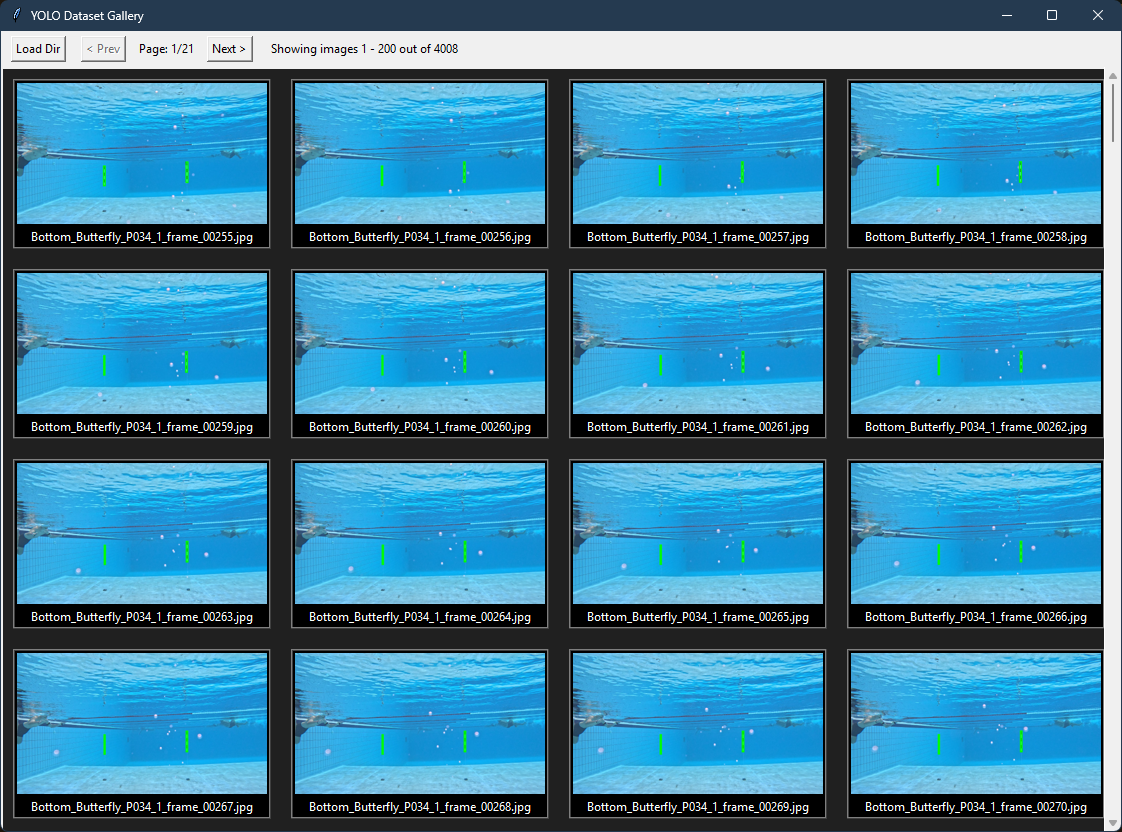
\includegraphics[width=0.8\textwidth]{bbox_editor.png}
    \caption{Human-in-the-loop verification tool interface for annotated bounding boxes.}\label{fig:bbox_editor}
\end{figure}

The interface displayed all the video frames with their bounding boxes overlaid, allowing the user to quickly navigate through the entire dataset. The user could click on any frame to maximize it, and then manually add, remove, or adjust bounding boxes as needed. This step was crucial for catching any remaining errors that automated filtering might have missed, such as subtle mask bleed or borderline identity switches that did not trigger the \gls{iqr} outlier detection. Thanks to the initial filtering, the main use of this tool was to manually add bounding boxes for frames where \gls{sam} 2 failed to detect a marker at all, which is a critical failure mode for scale estimation since it reduces the number of visible reference pairs. The tool's design prioritized efficiency, allowing the user to audit thousands of frames in a matter of hours, thus ensuring that the final training set was of the highest possible quality before being used to train the \gls{yolo26}s model.
This hybrid approach of combining foundation model automation with human oversight exemplifies the \gls{mitl} paradigm, leveraging the strengths of both machine and human intelligence to create a robust dataset for training a precision detection model. This step was crucial for establishing a ground truth
used for the final model fine-tuning and the subsequent accuracy evaluations in Chapter~\ref{chp:evaluation}.


% ============================================================
\section{Dynamic Scale Extraction Pipeline}\label{sec:scale-extraction}
% ============================================================

Objective~\ref{obj:calibration} focuses on establishing a stable reference for converting image coordinates into
metric units.

\subsection{Model Selection Rationale}

Before describing the training configuration, it is necessary to justify the choice of \gls{yolo26}
over alternative detection architectures. Two-stage detectors such as Faster \gls{rcnn} achieve
higher accuracy on standard benchmarks by separating region proposal from classification, but
their inference speed is incompatible with the requirement to process full video sequences at
interactive rates. For a single-class detection task on visually distinctive markers, a
one-stage \gls{yolo} variant provides sufficient localization accuracy at a fraction of the
computational cost, making the accuracy-throughput trade-off clearly favourable for the
proposed pipeline. Among the \gls{yolo} family, earlier versions such as v7, v8, and v10 were
considered but \gls{yolo26} was selected for its improved small-object detection head and its
anchor-free regression formulation, which is better suited to cylindrical targets whose
bounding box aspect ratios vary continuously with viewing distance rather than clustering
around a few predefined anchor aspect ratios.

\subsection{Marker Detection via \gls{yolo26}}

A custom \gls{yolo26}s model~\cite{jocher_ultralytics_2023} was fine-tuned on the \gls{sam}-generated
dataset to provide a robust method for localizing markers. To ensure high localization
accuracy, which is critical for the subsequent pixel-to-metre ratio calculation, the training
process utilized a \gls{dfl} gain of $1.5$ and a Box Loss gain of $7.5$.
These settings prioritize bounding box regression over classification accuracy, as the project
involves a single-class detection task where classification loss is trivially small and
allocating representational capacity to it would be wasteful: upweighting the box regression
terms forces the model to refine its localization precision, which is the property that
directly governs the accuracy of the scale calibration downstream.

Training was conducted over 200 epochs with an image resolution of $640 \times 640$ pixels.
Higher resolutions were considered but rejected on the grounds that the markers occupy
sufficient pixels at 640 that sub-pixel localization precision is not the limiting factor in
scale estimation, and the associated increase in \gls{gpu} memory consumption would have required
reducing the batch size, adversely affecting gradient estimate quality. To mitigate overfitting
on the \gls{sam}-generated dataset, several regularization and augmentation strategies were
employed.

An initial learning rate of $0.01$ was used with a 3-epoch warm-up period and a momentum of
$0.937$ to stabilize early gradient descent, preventing the large gradient steps in the
initial epochs from perturbing the pre-trained feature representations before the learning
rate scheduler had converged. 

The model utilized Mosaic augmentation ($1.0$) and Random
Erasing ($0.4$) to simulate occlusions and varying marker densities, forcing the network to
learn robust features rather than memorizing specific marker placements. Mosaic augmentation
directly addresses the scenario where markers appear at different apparent scales within the
same field of view, as occurs when the camera is closer to some markers than others along the
lane. Random Erasing simulates transient occlusions caused by splashing water, training the
model to produce valid detections even when part of the marker is obscured. 

Variations in
lighting and glare were accounted for by adjusting \gls{hsv} gains
($hsv\_h=0.015$, $hsv\_s=0.7$, $hsv\_v=0.4$). The saturation jitter value of $0.7$ is
intentionally high because pool environments vary dramatically in colour temperature between
outdoor venues under natural daylight and indoor venues under fluorescent or LED illumination,
and the model must remain effective across this range without retraining. 

An early stopping patience of $20$ epochs was implemented to terminate training if the validation fitness failed to
improve, providing an automatic mechanism for balancing the risk of underfitting at low epoch
counts against the risk of overfitting at high epoch counts given the limited dataset size.

Training was performed on a \gls{cuda}-capable \gls{gpu}, and the resulting model outputs high-confidence
bounding boxes that serve as the foundation for physical distance estimation, leveraging the
known dimensions of the physical markers to establish spatial scale.

The small (s) variant was selected over the nano (n) and medium (m) alternatives
based on the A/B experimental results from Section~\ref{sec:dataset-generation}. The nano
model demonstrated a non-trivial false negative rate on partially occluded markers, which
constitutes the critical failure mode for scale estimation, since a missed marker reduces the
number of visible reference pairs. The medium model offered negligible improvement in recall
over the small variant while approximately doubling inference time, making the small variant
the optimal point on the accuracy-throughput trade-off curve for this application.

\subsection{Refraction-Aware Scaling}

As identified in preliminary experiments, frame-independent scaling is susceptible to
refractive noise. To stabilize the scale, the system implements a \gls{mad} inlier mask~\cite{leys2013detecting}. This filter calculates the pixel-to-metre ratio
($px/m$) for all visible marker pairs and rejects outliers that deviate by more than $k$ times
the \gls{mad} from the median, where $k$ was set to accommodate the expected variance in
refraction-induced scale jitter while retaining the majority of valid observations. The \gls{mad}
was preferred over the \gls{iqr} for this inference-time filtering task because the number of visible
marker pairs per frame can be very small, making the \gls{iqr} either
undefined or unreliable at such small sample sizes, whereas the \gls{mad} operates on the
point-wise distribution of per-pair ratios and remains statistically valid even with a handful
of observations. This ensures a stable calibration constant $C$ for each frame.

When fewer than two markers are simultaneously visible, it is impossible to compute an
inter-marker distance and therefore impossible to derive a fresh scale estimate. In this case,
the most recent valid ratio $\rho$ is carried forward to the current frame. This introduces a
risk of temporal staleness: if the swimmer moves significantly in depth between calibration
frames, the apparent size of the markers changes and the carried-forward $\rho$ becomes
inaccurate. This risk was accepted as a pragmatic trade-off given the typical geometry of
poolside filming, where depth variation is small relative to the camera-to-lane distance and
the resulting scale error is therefore bounded. The carry-forward mechanism is analogous to the
zero-order hold in control systems and is a standard approach in tracking pipelines where
sensor observations are intermittent.

% ============================================================
\section{Kinematic Metric Extraction}\label{sec:kinematic-extraction}
% ============================================================

The final phase (Objective~\ref{obj:kinematic_metrics}) synthesizes the outputs of marker detection, ego-motion compensation, and pose
estimation to produce absolute positional and kinematic metrics for the swimmer.

\subsection{Ego-Motion Compensation}

Because the camera is hand-held and moved manually alongside the swimmer, raw pixel coordinates
are subject to both lateral drift and incidental shake between frames, making them incomparable
across time without compensation. The choice of handheld video over a fixed camera installation
was a deliberate architectural decision rather than a pragmatic compromise. A fixed camera
would eliminate the need for ego-motion compensation entirely, but it would cover only a
fraction of the lane from a single vantage point, requiring either multiple synchronized
cameras or an acceptance that the majority of the swim would not be monitored. The handheld
approach requires no permanent poolside infrastructure, making the system deployable at any
competition or training venue without modification to the facility. The operator can pan or move the camera to keep the swimmer in frame throughout the full length of the pool, and it reflects the realistic
data collection scenario facing a coaching practitioner without access to dedicated multi-camera
installations.

To recover an absolute reference frame, the system exploits the lane markers as stationary
anchors. For each consecutive frame pair, the horizontal pixel displacement of each detected
marker is computed and matched to the nearest marker in the previous frame within a 50-pixel
tolerance window. At the nominal pixel-to-metre ratio observed during trials, a 50-pixel
window corresponds to a physical distance sufficient to accommodate the inter-frame camera
displacement produced by typical handheld movement, while remaining small enough to prevent a
marker in one position from being incorrectly matched to a different marker at the adjacent
lane boundary. The median of all valid per-marker displacements gives a robust estimate of the
camera's pixel shift $\Delta x_{\text{cam}}$, which is accumulated into a running global offset
$X_{\text{cam}}$. The median is used in preference to the mean because the camera's motion is
not uniform: brief sharp jolts from the operator's stride produce a non-Gaussian jitter
distribution with heavy tails, for which the median is the appropriate central estimator:

\begin{equation}
    X_{\text{cam}}^{(t)} = X_{\text{cam}}^{(t-1)} - \Delta x_{\text{cam}}^{(t)}
\end{equation}

If no markers are detected in a given frame, the previous frame's displacement estimate is
propagated forward (linear projection), preventing a discontinuity in the accumulated offset.
The global pixel position of the swimmer is then:

\begin{equation}
    p_{\text{global}} = p_{\text{pixel}} + X_{\text{cam}}
\end{equation}

Where $p_{\text{pixel}}$ is the swimmer's raw horizontal pixel coordinate in the current frame.

Feature-based optical flow, specifically the Lucas-Kanade tracker, was evaluated as a
classical alternative for ego-motion estimation. However, the pool environment's repetitive
textures generate numerous ambiguous feature matches that violate the spatial smoothness assumption
underpinning optical flow methods. Electronic image stabilization, available in some consumer
cameras, was considered as a hardware-level alternative but was unavailable on the recording
hardware used in this project. The marker-based approach is semantically grounded in the
geometry of the scene and is therefore more reliable in the repetitively textured aquatic
environment than gradient-based feature matching.

\subsection{Metric Scale Calibration}

The pixel-to-metre conversion factor $\rho$ ($px/m$) is estimated from the detected marker
positions in each frame. Given $N$ markers detected and sorted left-to-right, the outermost
pair spans $N-1$ physical intervals of known separation $d_{\text{real}}$ (metres). The scale
is therefore:

\begin{equation}
    \rho = \frac{\lVert \mathbf{p}_N - \mathbf{p}_1 \rVert_2}{(N-1)\, d_{\text{real}}}
\end{equation}

\noindent Where $\mathbf{p}_1, \mathbf{p}_N \in \mathbb{R}^2$ are the pixel coordinates of the
leftmost and rightmost detected markers respectively, and $\lVert \cdot \rVert_2$ denotes the
Euclidean distance between them in the image plane.

The estimate from the most recent frame in which two or more markers are visible is carried
forward to frames where the marker count drops below two. The swimmer's absolute position in
metres is then:

\begin{equation}
    x_{\text{m}} = \frac{p_{\text{global}}}{\rho}
\end{equation}

\subsection{Swimmer Localization via ViTPose}

The swimmer's position is localized using the ViTPose pose estimation model~\cite{xu2022vitpose}.
ViTPose was selected over two principal alternatives. The OpenPose bottom-up approach~\cite{cao2019openpose}
was evaluated during preliminary testing but was found to fail frequently when a swimmer's
limbs crossed the water-air boundary, as the part affinity field grouping mechanism relied on
localized gradient features that are disrupted by refraction and surface glare at this
interface. \gls{hrnet}-based top-down models~\cite{wang2020deep} were considered as a technically
competitive alternative, however, ViTPose's plain \gls{vit} backbone~\cite{dosovitskiy2020image}
offers a specific advantage in the aquatic domain: its global self-attention mechanism
aggregates contextual information from the full image at every layer, allowing the model to
infer a joint's position from the broader kinematic context of the body even when that joint
is locally indistinguishable from the water surface. This global receptive field is
architecturally absent in convolutional \gls{hrnet} variants, which rely on local convolutions and
can be confused when localized keypoint evidence is obliterated by water.

A commonly used alternative for pose estimation in real-time applications is MediaPipe Pose, which provides efficient, lightweight keypoint detection suitable for mobile and embedded systems. However, MediaPipe is validated primarily on standard terrestrial datasets featuring stable lighting and limited occlusion. In the aquatic domain, where body parts are frequently obscured by splashes, bubbles, and refraction effects, its performance can degrade significantly due to its reliance on local feature consistency and vulnerability to severe frame degradation and visual noise~\cite{elshami2025visual}. In contrast, ViTPose leverages a non-hierarchical, vision transformer-based architecture. This global self-attention mechanism allows it to maintain structural integrity and handle complex, degraded, or blurry scenes by utilizing contextual information from the full body. Consequently, ViTPose is highly suitable for the challenging visual conditions encountered in swimming footage, where structural robustness is prioritized over real-time performance.

Rather than using the bounding box centroid, the system extracts the left and right hip
keypoints (\gls{coco} indices 11 and 12) and computes their midpoint as a proxy for the \gls{com}:

\begin{equation}
    \mathbf{c}_{\text{hip}} = \frac{\mathbf{k}_{11} + \mathbf{k}_{12}}{2}
\end{equation}

The biomechanical rationale for this choice is that the \gls{com} of a swimmer is located
near the pelvis and hip region throughout all stroke phases. Using the bounding box centroid
as a position proxy introduces a systematic error: during the arm entry phase of the stroke
cycle, the extended arm shifts the bounding box centroid forward by a body-length fraction,
introducing an artificial velocity oscillation at the stroke frequency that would contaminate
the kinematic profile. The hip midpoint is anatomically stable relative to the true \gls{com} across
all stroke phases and is therefore a more appropriate proxy for a quantity intended to reflect
whole-body translation. To account for any lateral offset between the swimmer and the marker
baseline, the hip centroid is orthogonally projected onto the line segment connecting the
outermost detected markers before the position is converted to metres.

Wrist keypoints (\gls{coco} indices 9 and 10) are additionally extracted with a confidence threshold
of $0.3$, providing left- and right-wrist positions in the global reference frame for
downstream stroke-cycle analysis. The lower confidence threshold for wrists relative to hips
reflects the deliberate asymmetry in their detectability: the hips are typically below the
waterline and visible throughout the stroke in underwater video, while the wrists are frequently lifted out of the water, or occluded by splashes, causing ViTPose to assign lower confidence scores to anatomically valid detections. Retaining low-confidence wrist detections accepts a degree of additional noise in exchange for improved recall of true positive wrist positions, a trade-off that is appropriate because wrist data is
used for qualitative stroke analysis rather than as the primary input to the position tracking
pipeline.

\subsection{Velocity and Kinematic Profile Extraction}

The raw per-frame position records are first subjected to a \gls{mad}
outlier filter and a temporal jump filter to remove implausible discontinuities. The \gls{mad}
pre-filter is applied before the Kalman filter rather than relying on the filter alone because
the Kalman filter's Gaussian noise model is not robust to large impulsive errors: a gross
outlier, such as a pose estimation failure that places the hip keypoint at the edge of the
frame, will corrupt the Kalman state estimate for several subsequent frames before the
innovation sequence recovers. Removing such gross errors prior to ingestion into the filter
preserves the integrity of the state estimate throughout the trajectory.

The cleaned trajectory is then processed by a discrete-time Kalman Filter~\cite{kalman1960new},
which models the swimmer as a constant-velocity system and simultaneously estimates position
and instantaneous velocity from the noisy observations. The constant-velocity model is
appropriate for the steady-state phase of a swim length, where accelerations between
consecutive frames are small relative to the observation noise. It would be less appropriate
at push-off or at the turning wall, where the swimmer undergoes rapid acceleration. A particle filter was considered as an alternative smoother for
cases where the position distribution is multi-modal, but the swimmer's position distribution,
conditioned on recent observations, is approximately Gaussian in the single-lane tracking
scenario, making the Kalman filter optimal in the least-squares sense and computationally
far less expensive. The process noise covariance $Q$ encodes the expected acceleration
variance between frames ($\sigma^2_a = 3.0\ \text{m}^2\text{s}^{-4}$), and the observation
noise covariance $R$ encodes the estimated metric-space position noise of the ViTPose hip
detection after scale calibration ($\sigma^2_\text{obs} = 0.015\ \text{m}^2$).

Following Kalman filtering, a loop closure correction is applied to the estimated position
track. Because scale calibration errors accumulate over the course of a length, the Kalman
position estimate at the turning wall may not coincide precisely with the known pool dimension
of 25 m. The correction rescales the outbound and return segments of the position track
piecewise so that the peak of the trajectory aligns exactly with 25 m, enforcing physical
consistency with the pool geometry. This step operates on the complete trajectory and is
therefore a batch post-processing operation rather than a causal one as it cannot be performed
until all frames have been processed.

Instantaneous velocity is then derived from the loop-closure-corrected position via numerical
differentiation:

\begin{equation}
    v(t) = \frac{\mathrm{d}}{\mathrm{d}t}\left(\frac{p_{\text{global}}(t)}{\rho}\right)
\end{equation}

Numerical differentiation amplifies high-frequency noise in the position signal, necessitating
a dedicated smoothing stage. A Savitzky-Golay filter is applied to the differentiated velocity
signal, with a window length of 61 frames and a polynomial order of 3 for the hip centroid
velocity. The Savitzky-Golay filter is well suited to this role precisely because, at this
stage of the pipeline, all frames are available: unlike the Kalman filter, it is a batch
operation and requires a symmetric window of neighbouring frames, which makes it inappropriate
for causal position tracking but entirely appropriate for this final offline smoothing step.
Its polynomial-fitting formulation preserves the shape of genuine kinematic events such as
velocity peaks and stroke-cycle troughs more faithfully than a simple moving average, which
would attenuate such features in proportion to their sharpness.

For wrist velocity signals, an extended cleaning pipeline is applied before the Savitzky-Golay
smoothing stage: biological thresholding removes physically impossible velocity values,
linear interpolation fills the resulting gaps produced by \gls{nan}-valued frames where the wrist
keypoints were not detected, and a median filter suppresses residual impulse noise before the
Savitzky-Golay filter is applied with a shorter window of 15 frames. The shorter window
reflects the higher temporal frequency of the wrist motion relative to the whole-body
translation of the hip centroid.

From the smoothed velocity estimates, summary kinematic metrics are derived: absolute speed
profile, peak velocity, and mean velocity over the analysed swim segment.

% ============================================================
\section{Summary}\label{sec:methodology-summary}
% ============================================================

This chapter presented a four-phase methodology for extracting swimmer kinematics from
handheld poolside video, in which each phase was designed not in isolation but to address the
specific error mode introduced by the preceding phase's output. The modular 3D-printed marker
system was designed to remain visually identifiable under the refractive and turbulent
conditions of the aquatic environment, with the alternating binary pattern and cylindrical
geometry chosen to overcome the contrast and viewpoint-sensitivity failure modes that preclude
the use of conventional planar calibration targets.

Manual annotation was rejected as
intractable at scale, synthetic generation as insufficiently realistic, and direct transfer
learning as impractical in the absence of domain-matched public data. The \gls{mitl}
pipeline, combining \gls{sam} 2 propagation with \gls{iqr}-based outlier filtering and human verification,
was therefore developed to construct a domain-specific training set at manageable cost. A
refraction-aware \gls{mad} inlier filter was applied to stabilize the per-frame pixel-to-metre scale
estimate derived from the known marker spacing, with the \gls{mad} selected over the \gls{iqr} specifically
because it remains valid when the number of observable reference pairs is small.

Finally,
ego-motion compensation using the markers as stationary anchors, ViTPose-based hip
localization selected for its global attention mechanism and anatomical proximity to the centre
of mass, and a Kalman filter smoothing stage were combined to produce absolute positional and
velocity profiles from the raw tracking output. Feature-based optical flow was rejected for
ego-motion estimation due to the repetitive textures of the pool environment, OpenPose was
rejected due to its failure at the water-air boundary, and the particle filter was rejected on
grounds of computational overhead given the approximately Gaussian position distribution. The Kalman filter handles causal position tracking, a loop closure step corrects
accumulated scale error against the known 25 m pool geometry, and the Savitzky-Golay filter
then smooths the velocity signal produced by numerical differentiation of the corrected
trajectory, a role for which its non-causal polynomial formulation is well suited.

The system described in this chapter constitutes a complete pipeline from physical marker
placement to calibrated kinematic output. Chapter~\ref{chp:evaluation} evaluates each
component against quantitative accuracy benchmarks and characterizes the residual error sources
that remain after the mitigation strategies described here have been applied.
